\section{DisasterClaw benchmark construction}
\label{sec:benchmark}
The benchmark converts registered disaster records into questions whose answers are computed from annotations and geometry before any agent is evaluated. A task is not simply an image--text pair: it binds a question to a geographic ROI, an initial vehicle state, an answer vocabulary, and a reference answer that remains fixed as the agent moves. Table~\ref{tab:benchmark-summary} summarizes the final set and distinguishes its size from the number of executed episodes.

\begin{table}[htbp]
\centering\small
\caption{Final benchmark and execution scope. Repeated policy runs do not increase the number of independent questions or source regions.}
\label{tab:benchmark-summary}
\begin{tabularx}{\linewidth}{@{}p{0.28\linewidth}X@{}}
\toprule
Item & Specification \\
\midrule
Source evidence & Paired xBD imagery, registered building polygons, and damage labels \\
Final task set & 160 questions over 44 geographic ROIs from three events \\
Event composition & Hurricane Michael: 48; Moore tornado: 51; Nepal flooding: 61 questions \\
Task families & Presence, damage, count, and spatial relation \\
Reference answers & Deterministic annotation and geometry rules; no LLM-generated ground truth \\
Label space & Binary no-damage/damaged; count buckets $0,1,2,3+$; eight compass directions \\
Quality control & Coverage and split checks, schema/answer checks, duplicate detection, ambiguity flags \\
Human review & Two independent reviews and disagreement adjudication before freezing \\
Online evaluation & Seven policies $\times$ 160 questions $\times$ three repeats = 3,360 episodes \\
\bottomrule
\end{tabularx}
\end{table}

\subsection{Source records and candidate ROI selection}
Candidate records require a post-disaster image, a usable geographic footprint, and the corresponding label file. Paired pre-disaster imagery supplies the archival reference used by the damage-perception pipeline. The ROI index evaluates whether available georeferenced post-disaster tiles cover the configured cruise observation footprint. The generator's default minimum coverage is 0.80: this is the fraction of that observation footprint supported by disaster imagery, not a requirement that a task ROI contain 80\% buildings or that 80\% of the ROI be damaged.

Valid building records provide a polygon, a geographic centroid, a source identifier, and one of the four supported xBD damage labels. For the binary benchmark, minor damage, major damage, and destroyed are mapped to damaged; no-damage is retained as the other class. Unclassified or unusable records do not define binary reference answers. Source polygons and damage labels are used for task construction and scoring, not shown as ground-truth overlays to the evaluated agent.

\subsection{Event split and geographic ROI construction}
The generator selects eligible records from the configured evaluation events, excludes tile identifiers already recorded in the consumed-ROI registry, and uses seeded shuffling with round-robin selection across events. A tile can yield up to four task families subject to their prerequisites. Consequently, the final 160 questions are neither 160 independent tiles nor necessarily 40 questions per family. The observed event counts are reported in Table~\ref{tab:benchmark-summary} rather than described as an exactly balanced allocation.

Each question stores its source tile identifier, geographic ROI bounds and center, and initial latitude, longitude, and altitude. A building belongs to the reference ROI when its centroid lies within the closed ROI bounds. Let $B_R$ be this building set and $D_R\subseteq B_R$ its damaged subset. Reference answers are defined on this fixed geographic region, not on whichever crop happens to be visible at a later step. The consumed-record check separates the final task ROIs from development use; it does not establish event-disjoint pretraining for the fixed ChangeOS checkpoint.

\subsection{Programmatic task and answer generation}
Questions are instantiated from task templates, while reference answers follow explicit rules:
\begin{itemize}
\item \textbf{Presence:} whether a damaged building exists in the ROI, with answer $\mathbf{1}[|D_R|>0]$. Positive evidence can settle an existence question, whereas a negative answer requires adequate regional coverage.
\item \textbf{Damage:} whether a designated building is damaged. A valid source building is selected, its identifier and location define the target, and its binary annotation determines the answer. The visible target cue identifies what to inspect; it does not expose the damage label.
\item \textbf{Count:} the number of damaged buildings in the ROI, mapped to $0$, $1$, $2$, or $3+$. This requires maintaining the regional extent and avoiding duplicate counting across views.
\item \textbf{Spatial:} the compass direction from the ROI center to the nearest damaged building. Distance is computed in a local metric north--east frame; bearing is quantized into eight 45-degree sectors. This task requires a nonempty $D_R$ and preserves an explicit geographic reference point.
\end{itemize}
No language model supplies the ground-truth answer. The task schema also retains answer choices, target metadata when applicable, and geometric difficulty or ambiguity indicators. Such indicators describe construction conditions, such as nearby candidates or boundary proximity; they are not measurements of agent difficulty or evidence of balanced difficulty strata.

\begin{figure}[htbp]
\centering
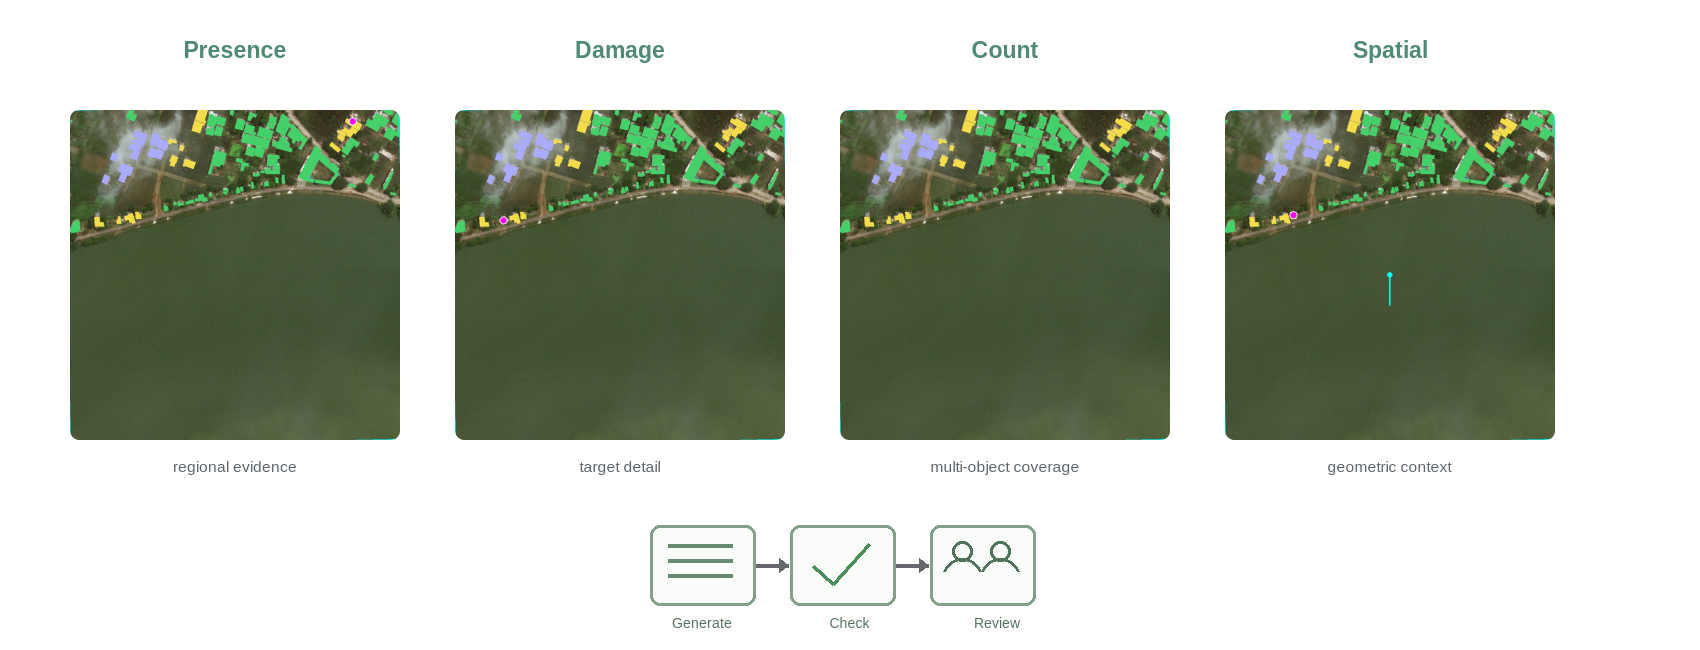
\includegraphics[width=\linewidth]{figure-paper/Fig3_Task_Benchmark.png}
\caption{Illustrative spatial evidence for the four task families. Presence concerns existence within a region, damage concerns a designated building, count concerns region-wide aggregation, and spatial questions concern a target's direction relative to a geographic reference. These supplied panels illustrate task construction; they do not provide verified question--answer pairs from the frozen 160-question set. Colored polygons and markers are construction overlays, not ground-truth inputs to the agent.}
\label{fig:benchmark-tasks}
\end{figure}

\subsection{Automated quality control}
Generation and review checks cover required fields and answer vocabularies, geographic validity, consistency of answers with annotations and geometry, the binary label mode, event membership, and previously consumed records. Duplicate checks use the source tile, task type, question text, and answer. Geometric ambiguity notices are retained for review rather than interpreted as an automatic guarantee that a question is visually answerable. Records that fail acceptance checks require correction and renewed validation before inclusion in a frozen evaluation set.

The runtime task context contains the permitted question, ROI, initial state, and target cue. Reference labels and answer fields remain in the evaluation path. This separation matters because the same source annotations support both world inspection by an operator and benchmark scoring; displaying an overlay in the console does not authorize providing it as agent evidence.

\subsection{Dual review and benchmark freezing}
Two annotators independently reviewed the 160 final questions for task type, ROI, target identity where applicable, reference-answer consistency, and answerability from the registered imagery and annotations. Disagreements were resolved before freezing; ambiguity notices were retained in the audit trail. Human review checks the applicability and clarity of the programmatic reference rather than replacing it with a language-model answer.

The final task set is distinct from the 160-question development set used to select policy rules. Once frozen, question identifiers and answers are shared across all policies and repeats. The execution protocol records task and review inputs together with source, prompt, checkpoint, and configuration identities. The locally available protocol and the remaining review-artifact release requirements are distinguished in \ref{app:provenance}. Neither dual review nor deterministic answers remove all annotation error or language-template shortcuts; these remain limitations of the benchmark.
